%\documentclass{hotnets22}
% \documentclass[sigconf,10pt]{acmart}
\documentclass[letterpaper,twocolumn,10pt]{article}
\usepackage{usenix-2020-09}
\usepackage{amsmath}

\usepackage{times}  
\usepackage{hyperref}
% \usepackage{subfig}
\usepackage{tikz}
\usetikzlibrary{math}
\usepackage{pgfplots}
\usepackage{pgfplotstable}

\usepackage{subcaption}
\usepackage{multirow}
\usepackage{tabularx}

\newcolumntype{s}{>{\hsize=.3\hsize\linewidth=\hsize}X}
\newcolumntype{D}{>{\hsize=.3\hsize\linewidth=\hsize}X}

\newcommand{\wdImg}{\dimexpr \linewidth-2\tabcolsep} %width of the image

\hypersetup{pdfstartview=FitH,pdfpagelayout=SinglePage}

\setlength\paperheight {11in}
\setlength\paperwidth {8.5in}
\setlength{\textwidth}{7in}
\setlength{\textheight}{9.25in}
\setlength{\oddsidemargin}{-.25in}
\setlength{\evensidemargin}{-.25in}

\newcommand{\rg}[1]{\textcolor{blue}{(\textbf{GR:} #1)}}

% TODO: remove for the CR!
% \pagestyle{plain}
% \settopmatter{printfolios=true}

\begin{document}

% \conferenceinfo{HotNets 2022} {}
% \CopyrightYear{2022}
% \crdata{X}
% \date{}

%%%%%%%%%%%% THIS IS WHERE WE PUT IN THE TITLE AND AUTHORS %%%%%%%%%%%%

\title{Beyond Amdahl's Law: Achieving Superlinear Scaling with\\Distributed Self-adjusting Systems}

\author{Paper \#??} %, 6 + 1 pages}

\maketitle

%%%%%%%%%%%%% ABSTRACT GOES HERE %%%%%%%%%%%%%%
\begin{abstract}
  Conventional wisdom suggests that doubling the number of workers in a distributed system can result at most 2x performance improvement, but most often less if the system does not provide perfect parallelism.  This common wisdom is codified by Amdahl's famous scaling law, asserting sublinear scaling and diminishing returns for parallelization. Several reports have indicated faster-than-linear (superlinear) scaling for various distributed applications, but most were dismissed as use-case specific artifacts, elusive interplays between memory and CPU, or mere measurement errors.

  In this paper we present the first systematic methodology to architect distributed systems to achieve superlinear scaling. Our key insight is that dispatching jobs to workers so that the locality of reference in the per-worker input streams increases, combined with self-adjusting workers that can take advantage of the higher locality to improve their own performance, yield faster-than-linear scaling. Using various off-the-shelf load balancing policies and self-adjusting algorithms from the literature, we report 100--1000x speedup when scaling certain distributed list lookup and tree search workloads to 36 CPU cores, up to 50x beyond what is predicted by Amdahl's law.  Surprisingly, we obtain nonzero scaling even when we keep the total computing power available to the system constant. By implementing an earlier self-adjusting packet classification algorithm in the Linux kernel and combining it with a simple hash-based RSS load balancer, we obtain 131x speedup on 20 cores for synthetic and 80x speedup for realistic firewall traces, 4.5x--6.3x performance improvement compared to Amdahl scaling and the default Linux packet classifier.
\end{abstract}

% \tableofcontents

% a unique combination of \emph{locality-boosting load balancing} to spread load among workers implemented using \emph{self-adjusting data structures}.
  
\section{Introduction}\label{sec:introduction}

With the end of Moore's law, computing power in modern systems increasingly comes in the form of parallel processing resources.  A major obstacle faced by network engineers is how to harness this increasingly parallel computing power for scaling distributed systems \cite{265065, 10.5555/3307441.3307467, 10.1145/2815400.2815423, 10.1145/3098822.3098826, 10.5555/3154630.3154639}.

In horizontally scaled applications, a load balancer dispatches jobs across a fleet of workers that process the jobs in parallel \cite{10.5555/3235491}.  In the context of \emph{web applications}, HTTP load balancers \cite{194966, 211279, 9552525} distribute requests across a swarm of backend web servers.  % by hashing over the source IP address (``sticky sessions'').
% This way, requests from the same client will hit the same backend server, improving request locality.
% Meanwhile, resource state is maintained in a key-value store or a relational database.
Multicore \emph{OS network stacks} \cite{211263, 10.1145/3359989.3365412, 10.1145/3452296.3472914} run multiple instances of the networking logic on different CPUs and leverage the NIC to dispatch packets to CPU cores. % In order to avoid packet reordering and improve CPU cache performance, the NIC typically computes a hash over the packet header fields to select the CPU (RSS, RPS, etc.).
In massive-scale \emph{key-value stores} \cite{ghigoff2021bmc}, the key-space is hashed into multiple shards (partitions) and each shard is assigned to a separate server for processing.  The system's overall goal is to achieve the greatest possible parallel speedup with a given number of workers, in order to minimize the execution time of a single task or maximize the number of completed tasks in a given time period.

Suppose a web app handles 100 requests per second using a single server. As we add another server, we expect a throughput of 200 requests per second. In reality, however, we usually obtain slightly less, and this is worsened as the system is scaled up further. This is because some fraction of most workloads is inherently sequential and, therefore, bound to execute on a single CPU core. For instance, the web servers may need to synchronize on a mutex to access global state, which makes all state updates sequential.  Beyond a certain threshold parallel performance plateaus as the sequential workload becomes a bottleneck.

The maximum speedup, measured as the ratio of the wall clock times of sequential and parallel execution, is formally described by Amdahl's law \cite{10.1145/1465482.1465560}. In general, the greater the sequential portion compared to the parallelizable fraction of the code, the more performance is lost compared to an ``ideal'' linear scaling, and the faster the system reaches saturation (see Fig.~\ref{fig:amdahl}). Amdahl's law is a cornerstone result in the parallel and high-performance computing practice and, despite often being debated \cite{10.1145/42411.42415}, extended \cite{4563876, 6280307,1580395,406581,6163449}, and misused \cite{10.5555/775339.775386}, it has remained one of the most useful tools in the system engineering toolbox \cite{10.5555/1951599}.

\begin{figure}[t]
  \centering
  % \includegraphics[width=0.8\linewidth]{fig/usl.png}
  \begin{small}
  \begin{small}
  \begin{tikzpicture}[remember picture]
    \begin{axis}[
      width=250pt,
      height=170pt,
      xlabel={\#threads},
      ylabel={Speedup},
      xlabel near ticks,
      ylabel near ticks,
      xmin=1,
      xmax=25,
      ymin=1,
      ymax=90,
      xtick={1,5,10,15,20,24},
      legend style = {
        anchor = north west,
        at = {(rel axis cs:0.01,0.98)},
        font=\scriptsize,
        % draw = none,
      },
      no markers
      ]
      % use TeX as calculator:
      \addplot[domain=1:25,black,densely dotted]{x};
      \addlegendentry{Linear scaling}

      \addplot[domain=1:25,black,densely dashed]{1/(0.01 + (1-0.01)/x)};
      \addlegendentry{Amdahl's law}

      \addplot[domain=1:25,black,solid]{1/(0.01 + (1-0.01)/x^2)};
      \addlegendentry{Proposed scaling law}

      \coordinate (insetPosition) at (rel axis cs:.97,0.25);
      % \addplot[domain=0:15,black,loosely dashed]{1/(0.4 + (1-0.4)/x)};
      % \addlegendentry{Amdahl's law ($\delta=0.4$)}

      % \addplot[domain=0:15,black,loosely dotted]{1/(0.4 + (1-0.4)/x^2)};
      % \addlegendentry{Proposed scaling law for MTF ($\delta=0.4$)}
    \end{axis}
    \begin{axis}[
      at={(insetPosition)},
      anchor={outer south east},
      width=105pt,
      height=85pt,
      tiny,
      % xlabel={\#cores},
      % ylabel={Speedup},
      xmin=1,
      xmax=450,
      ymin=0,
      ymax=110,
      % ytick={1,2,3,4,5},
      no markers]
      \addplot[domain=1:500,black,densely dotted]{x};
      \addplot[domain=1:500,black,densely dashed]{1/(0.01 + (1-0.01)/x)};
      \addplot[domain=1:500,black,solid]{1/(0.01 + (1-0.01)/x^2)};
    \end{axis}
  \end{tikzpicture}
\end{small}

%%% Local Variables:
%%% mode: latex
%%% TeX-master: "../distributed_mrf.tex"
%%% End:

\end{small}
  \caption{Linear scaling, Amdahl's law and the superlinear scaling ($s=0.01$). The inset shows the asymptotics.}
  \label{fig:amdahl}
\end{figure}

Inherent to Amdahl's law is that no system can scale faster than linear: doubling parallel resources will yield at most two times the performance. Curiously, there have been several reports on faster-than-linear (\emph{superlinear}) scaling experimentally observed in, e.g., database systems \cite{scalability-analyzed, 10.5555/1012889.1012894}, distributed caching \cite{271208, dobb-2}, SDN analytics \cite{sdn-analytitcs}, high-performance computing \cite{556383, 7733347, 6483679}, multi-robot systems \cite{10.1007/978-3-319-77610-1}, and parallel search in information retrieval systems \cite{dobb-1, dobb-2} (see full taxonomies in \cite{7733347, 80148}).
% There seem to be two ways to achieve such superlinear speedup \cite{7733347, 80148}: do disproportionately less work in each worker as we scale the system \cite{7733347}, or add more resources per thread \cite{80148}.
% One typical context in which superlinear growth often emerges is distributed caching \cite{271208, 10.5555/1012889.1012894, dobb-2}: the more CPU cores the more (unshared) L1 cache space available to the application, which tends to make memory-bound\slash cache-bound code disproportionately faster \cite{80148} (see an analysis in \S\ref{sec:background}).  
Many authors argue, however, that superlinear scaling is merely a byproduct of running memory-\slash cache-bound applications on a ``bigger machine'' \cite{80148}, others are concerned that it is hard to generalize beyond a specific set use cases \cite{7733347, 80148}, and some outright dismiss faster-than-linear scaling all together \cite{gunther-hotsos, 10.1016/0167-8191(86)90024-4}, concluding that \emph{``superlinearity, although alluring, is as illusory as perpetual motion''} \cite{10.1145/2773212.2789974}.

In this paper we challenge this view: we show that distributed systems can be methodologically designed for reaching superlinear scaling. Our motivation is that networking applications are often embarrassingly parallel, % with little or no dependency between parallel workers,
which may admit a massive superlinear initial growth phase before scaling eventually and unavoidably blocking on a serial bottleneck.

Our main observation is that, to achieve superlinearity, one has to carefully combine an appropriate load balancing policy with a proper worker implementation. Indeed, load balancing in most distributed systems is deliberately designed to improve the locality of reference in the input of the workers: web apps apply the ``sticky sessions'' rule to route all requests of a particular user to the same web server; %, rendering subsequent requests faster by having all per-user state available locally;
networking code often uses IP 5-tuple hashing on the NIC to ensure that all packets of a flow are processed on the same CPU; % that has local access to per-flow information;
and key-hashing in sharded key-value stores directs all client queries to a key to the same replica. Each of these load balancing policies tend to make the input stream processed by the parallel workers more predictable, compared to the input processed by the system. Such a \emph{locality boosting load balancer}, paired with a \emph{self-adjusting algorithm} so that workers can take advantage of the higher input predictability to adaptively improve their performance, will, as we show both theoretically and empirically, yield faster-than-linear speedup in a broad range of applications (see Fig.~\ref{fig:amdahl}). % One growth factor would come from the self-adjusting algorithm becoming proportionately faster as it processes a smaller and smaller subset of the inputs, and another factor would result from the fact that we throw more CPU resources to the system.

After some background on Amdahl's law (\S\ref{sec:background}), we present our \emph{distributed self-adjusting system architecture} and show that superlinear speedup is a natural product of combining locality-boosting load balancing with self-adjusting algorithms (\S\ref{sec:architecture}). Using common list and tree search algorithms from the literature, we achieve 100x--3300x speedup in simulations, orders of magnitude surpassing Amdahl's law or even plain, linear scaling. As an unexpected byproduct, we attain linear scaling even when we limit the system to a single CPU core. Then we extend our analysis to real systems (\S\ref{sec:case-study}): we carefully apply our methodology to engineer a Linux-kernel based packet classifier to reach superlinear scaling. On synthetic and real-life firewall traces, our implementation shows up to $800\times$ faster than linear scaling, $5\times$--$25\times$ improvement beyond the default Linux firewall implementation which scales according to Amdahl's law. Finally, we review related work (\S\ref{sec:related-work}) and draw the conclusions (\S\ref{sec:conclusions}). We note that all code will be available as open source after publication.

%%% Local Variables:
%%% mode: latex
%%% TeX-master: "distributed_mrf"
%%% End:



% !TEX ROOT = ./distributed_mrf.tex
\section{Background}\label{sec:background}

\begin{figure}[t]
  \centering
  \begin{small}
    \begin{small}
  \begin{tikzpicture}[remember picture]
    \begin{axis}[
      width=250pt,
      height=170pt,
      xlabel={\#threads},
      ylabel={Speedup},
      xlabel near ticks,
      ylabel near ticks,
      xmin=1,
      xmax=25,
      ymin=1,
      ymax=90,
      xtick={1,5,10,15,20,24},
      legend style = {
        anchor = north west,
        at = {(rel axis cs:0.01,0.98)},
        font=\scriptsize,
        % draw = none,
      },
      no markers
      ]
      % use TeX as calculator:
      \addplot[domain=1:25,black,densely dotted]{x};
      \addlegendentry{Linear scaling}

      \addplot[domain=1:25,black,densely dashed]{1/(0.01 + (1-0.01)/x)};
      \addlegendentry{Amdahl's law}

      \addplot[domain=1:25,black,solid]{1/(0.01 + (1-0.01)/x^2)};
      \addlegendentry{Proposed scaling law}

      \coordinate (insetPosition) at (rel axis cs:.97,0.25);
      % \addplot[domain=0:15,black,loosely dashed]{1/(0.4 + (1-0.4)/x)};
      % \addlegendentry{Amdahl's law ($\delta=0.4$)}

      % \addplot[domain=0:15,black,loosely dotted]{1/(0.4 + (1-0.4)/x^2)};
      % \addlegendentry{Proposed scaling law for MTF ($\delta=0.4$)}
    \end{axis}
    \begin{axis}[
      at={(insetPosition)},
      anchor={outer south east},
      width=105pt,
      height=85pt,
      tiny,
      % xlabel={\#cores},
      % ylabel={Speedup},
      xmin=1,
      xmax=450,
      ymin=0,
      ymax=110,
      % ytick={1,2,3,4,5},
      no markers]
      \addplot[domain=1:500,black,densely dotted]{x};
      \addplot[domain=1:500,black,densely dashed]{1/(0.01 + (1-0.01)/x)};
      \addplot[domain=1:500,black,solid]{1/(0.01 + (1-0.01)/x^2)};
    \end{axis}
  \end{tikzpicture}
\end{small}

%%% Local Variables:
%%% mode: latex
%%% TeX-master: "../distributed_mrf.tex"
%%% End:

  \end{small}
  \caption{Linear scaling, Amdahl's law and superlinear scaling ($s=0.01$). The inset shows the asymptotics.}
    \label{fig:amdahl}
\end{figure}

There is an extensive background on scaling laws for characterizing the performance of a parallel system as a function of the computing\slash storage capacity available to it. In the following, we will use the terms ``distributed'' and ``parallel'' interchangeably to connote a networked system scaled to multiple independent compute threads (``workers''), e.g., scaled to parallel CPUs of the same node, distributed to separate nodes, run in multiple datacenters, etc.

A cornerstone result in parallel computing, Amdahl's law \cite{10.1145/1465482.1465560} establishes a firm limit on the performance gain one can obtain by distributing a computation task over multiple processors. Given a partially parallel program, denote the fraction of execution time spent in the sequential part of the code by $s$, and the parallel fraction by $(1-s)$. Here, some code is ``sequential'' if it cannot benefit from the improvement of parallel computing resources, like single-threaded code, critical sections guarded by exclusion locks, etc. Denote by $T(k)$ the runtime (in seconds) of the program when executed on $k$ processors, and let $S(k)=\frac{T(1)}{T(k)}$ denote the performance improvement relative to a single-threaded execution (i.e., the \emph{speedup}). Then, the following holds (see Fig.~\ref{fig:amdahl}):
\begin{equation}\label{eq:amdahl}
S(k) = \frac{T(1)}{T(k)} = \frac{1}{s + \frac{1-s}{k}} \enspace .
\end{equation}

Here, $\frac{1-s}{k}$ establishes that the perfectly parallel part of the program executes $k$ times faster on $k$ processors than on a single core. By Amdahl's law, \emph{(i)} no code can scale faster than linear (i.e., $\frac{d S(k)}{d k} \le 1$, with equality exactly when $s=0$), \emph{(ii)} throwing additional workers on a computation task yields diminishing returns ($\frac{d S(k)}{d k}$ is monotonically decreasing in $k$) and \emph{(iii)} the asymptotics is limited by the sequential part only ($\lim_{k\to \infty}S(k) = \frac1{s}$). For different applications and extensions of Amdahl's law, see \cite{4563876, 6280307,1580395,406581,6163449, 10.5555/1951599}.

Curiously, there have been several reports from a broad range of applications indicating faster-than-linear scaling, e.g., database systems \cite{scalability-analyzed, 10.5555/1012889.1012894}, distributed storage systems \cite{271208, dobb-2, icsoft20}, SDN analytics \cite{sdn-analytitcs}, high-performance computing applications \cite{556383, 7733347, 6483679}, multi-robot systems \cite{10.1007/978-3-319-77610-1}, information retrieval systems \cite{dobb-1, dobb-2}, and large-scale network simulations \cite{10.1145/3627703.3629574} (see full taxonomies in \cite{7733347, 80148}). % (Note that in the majority of the literature any function growing faster than $f(x) = x$ is considered ``superlinear'', despite that, e.g., $f(x) = 3x$ is, mathematically, linear. Some authors distinguish these functions using the term ``superunitary'' \cite{80148}. In line with the literature we will use the former terminology below.)
One way to reconcile these empirical observations and Amdahl's law is the \emph{scaled size model} \cite{556383}. Critical to Amdahl's law is the assumption that the size of workers' sub-problems remains constant as we scale the system \cite{10.1145/42411.42415}. Under this \emph{fixed size} assumption \cite{556383}, faster-than-linear scaling is impossible \cite{10.1016/0167-8191(86)90024-4}. However, when this assumption fails, say, when the workers' jobs get progressively smaller or execution gets gradually faster as we add more parallel workers (scaled size model), superlinear scaling often emerges \cite{scalability-analyzed, sdn-analytitcs, 6483679, 10.1007/978-3-319-77610-1}.

Sometimes faster-than-linear growth appears almost accidentally. Imagine a naive parallel dense matrix-multiplication algorithm that factors input matrices into multiple blocks, performs the multiplication of the blocks in parallel, and aggregates the results \cite{7733347}. Easily, blocks will get smaller as we add more processors, so that after a certain point the entire input of workers will fit into CPU fast cache, yielding a disproportionately faster parallel execution. Conditions under which such superlinear (or ``super-unitary'' to be absolutely precise \cite{80148}) scaling emerges are widely discussed \cite{556383, dobb-1, dobb-2}, analyzed \cite{80148, 7733347}, and debated \cite{gunther-hotsos, 10.1016/0167-8191(86)90024-4, 10.1145/2773212.2789974}. What is missing is a generic design methodology to \emph{engineer} distributed systems for superlinear scaling. Such a model would also help identify the cases when superlinear scaling is possible, and when it is not. Our main contribution in this paper is a new system architecture to fill this gap.

% Many authors argue, however, that superlinear scaling is merely a~byproduct of running memory-\slash cache-bound applications on a ``bigger machine'' \cite{80148}, others are concerned that it is hard to generalize beyond a specific set use cases \cite{7733347, 80148}, and some outright dismiss faster-than-linear scaling all together \cite{gunther-hotsos, 10.1016/0167-8191(86)90024-4}, concluding that \emph{``superlinearity, although alluring, is as illusory as perpetual motion''} \cite{10.1145/2773212.2789974}.


% Currently the only general methodology to achieve faster-than-linear scaling seems to require deploying additional fast caches. Moving an application to a ``bigger machine'' \cite{dobb-2}, however, is not always feasible due to, e.g., physical or financial constraints.  In some cases caching cannot be used at all (e.g., for inherently stateful computations or complex database queries) or it introduces more overhead than it saves (e.g., for predominantly uniform input or rapidly changing data).  Moreover, caching comes with certain extra complexity and often cache invalidation and eviction policies and data consistency mechanisms are too costly to implement in a massively distributed setting \cite{271208}. Apart from caching, however, currently the only way to achieve faster-than-linear scaling is to rely on piecemeal problem-specific techniques, comprehensive domain knowledge, and pure luck \cite{7733347, 80148}. And even then, some compellingly argue that superlinear growth itself is a performance illusion, which goes against the very laws of nature much like perpetual motion \cite{gunther-hotsos, 10.1145/2773212.2789974}

% Many authors argue, however, that superlinear scaling is merely a~byproduct of running memory-\slash cache-bound applications on a ``bigger machine'' \cite{80148}, others are concerned that it is hard to generalize beyond a specific set use cases \cite{7733347, 80148}, and some outright dismiss faster-than-linear scaling all together \cite{gunther-hotsos, 10.1016/0167-8191(86)90024-4}, concluding that \emph{``superlinearity, although alluring, is as illusory as perpetual motion''} \cite{10.1145/2773212.2789974}.


%%% Local Variables:
%%% mode: latex
%%% TeX-master: "distributed_mrf"
%%% End:



\section{Distributed Self-adjusting Systems}
\label{sec:architecture}

Next we show a general distributed systems architecture, which, as we show theoretically and empirically later, produces faster-than-linear scaling in several disparate problem domains. Our main observation is that, whenever genuinely observed, superlinear scaling assumes two critical components: a policy to dispatch jobs to workers in a way to increase the locality of reference in the per-worker input streams, plus an algorithm that can adaptively exploit the structure in the input to process it more efficiently. Our architecture is a purely software technique and does not require, e.g., the addition of new cache memory to a system, but it contains distributed caching as a special case and hence automatically takes advantage of additional fast memory, if available.

\subsection{Locality-boosting load balancing}
\label{sec:lb-lb}

The first crucial component in our architecture is a locality-boosting load balancer.  In this context, load balancing refers to the distribution of computational work or incoming network traffic across multiple parallel workers (servers, processors, or nodes). A good load balancing strategy ensures optimal resource utilization, minimizes response time, avoids overloading any single resource, and, as we argue below, improves the locality in the input presented to the workers. 

In the context of this paper, \emph{locality of reference} is the property of a sequence of inputs that subsequent items are statistically dependent on each other. Such structure in the input can then be readily exploited by the proper algorithm \cite{SleatorT85Splay, BentleyCL93, HesterH85, HesterH85, BentleySTW86, Avin0020, ParkM12} or a runtime optimization framework \cite{276946,246322,10.1145/3503222.3507769,procieee_2019} to improve the performance of the code that processes it. A request set with minimal locality is uniformly distributed on the entire domain of possible inputs and hence unpredictable, while one with maximal locality contains only a single item, i.e., maximally predictable. A \emph{locality-boosting load balancing} policy is then a request dispatching strategy that can statistically or deterministically improve the locality of reference experienced by the worker threads, \emph{turning an unpredictable system input into multiple streams of predictable inputs to be processed by the workers} (see Fig.~\ref{fig:locality-boosting-lb}).

\begin{figure}
  \centering
  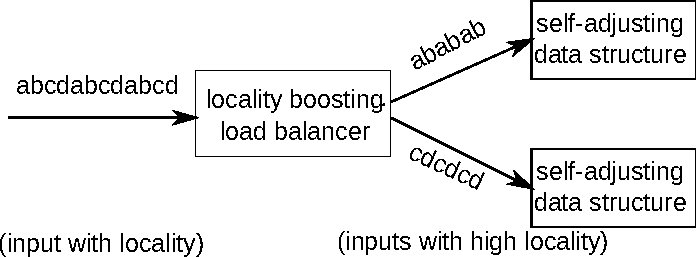
\includegraphics[width=.85\linewidth]{fig/schema.pdf}
  \caption{A locality boosting load balancer partitions the input sequence of a given locality into subsequences with higher locality. Self-adjusting data structures perform better on inputs with higher locality.}
  \label{fig:locality-boosting-lb}
\end{figure}

We distinguish two types of locality in this context. \emph{Spatial locality} means that the distribution of requested items on the entire input domain is statistically biased towards a particular subset of the items. One way to ensure this in the load balancer is to \emph{partition} the input domain into disjunct subsets, so that worker's input distributions are concentrated on a smaller set of inputs. For instance, the hash-based load balancer we used previously to show superlinear scaling with distributed caching is such a partitioning load balancer. In contrast, a round robin or a uniform random load balancer will export its own spatial input locality unchanged to the workers. A related concept is \emph{temporal locality}, which refers to the reuse of specific items in the input within a relatively small time duration. One way to boost temporal locality is to reorder items within a time window: e.g., Reframer applies controlled delays to particular packets in a packet batch to boost temporal locality and, thereby, enable more efficient processing \cite{276946,246322}.

\subsection{Self-adjusting algorithms}
\label{sec:sa-alg}

The second critical enabler for superlinear scaling in our architecture is \emph{self-adjusting algorithms}. Self-adjustment is a general term referring to the property of a dynamic data structure to \emph{automatically reorganize itself based on the sequence of operations it receives}, in order to optimize performance for future operations on frequently accessed or manipulated elements. Internal data reorganization always introduces extra complexity and overhead compared to a static data structure. Therefore, self adjustment can improve performance only if the input processed by the algorithm exhibits a certain amount of spatial or temporal locality.

Next we review the most prominent self-adjusting data structures (but see also \cite{BoseDL08, Avin0020, ParkM12}).

% For further examples, see self-adjusting skip lists~\cite{BoseDL08}, push-down trees~\cite{Avin0020}, or geometric data storages \cite{ParkM12}.

\noindent%
\textbf{Caches.} %
As the simplest but most universal self-adjusting data structure, caches can serve frequently accessed items fast by storing them in a  software or a hardware fast memory. This is typically much faster than if we had to run the request through the full processing pipeline or the slow backing store. Thus, caches have that almost magical capability of self-adaptation, without us having to engineer any prior knowledge of the input into the cache mechanism apart from a promise that it has nontrivial locality. When the promise is true, caches are an inexpensive way to improve throughput and response time. When there is no locality in the input, however, caches usually just add extra latency and overhead.
%
Note that caches do not necessarily have to come in the form of hardware memory: a fast key-value store is a candidate cache for a slow database \cite{10.5555/1012889.1012894}, a kernel fast-path flow cache is a useful way to speed up a slow user-space software switch \cite{188960}, etc.

% However, caches also come with additional complexity and overhead: cache entries have to be created for storing recently accessed data, invalidated when the backing data changes, evicted when the cache is full, and synchronized to consistently represent data that may be present in multiple caches. % Hardware implementations are appealing from this aspect by hiding the extra complexity behind a fast on-chip implementation.

% The performance of a cache is determined by the cache hit rate $\delta$, defined as the ratio of operations served from fast memory to those served on the slow path, and $\rho$, the penalty of a cache miss. In general, for a common LFU or LRU cache the higher the locality in the input and the bigger the cache compared to the input domain, the higher the cache hit rate and the lower the response time. When there is no locality in the input, caches usually just add extra latency and overhead.

\noindent%
\textbf{List lookup.} %
One of the most widely used self-adjusting data structures is the \emph{move-to-front list}. Suppose we wish to store a list of $m$ items in a way so that reordering, insertion and deletion are fast, while lookup is also reasonably efficient. A straightforward choice is a static (singly) linked list. Here, the cost of accessing an item at position $i$ is exactly $i$. Then, any linked list can easily be upgraded to a self-adjusting list using the move-to-front (MTF) heuristics: after accessing an item it is moved to the front, which improves lookup time for future requests of the same item at minimal cost (see Fig.~\ref{fig:mtf-example}). The MTF heuristics comes with appealing theoretical properties, namely that unconditionally moving the accessed item to the front of the list is close to the best one could achieve, even if one knew all future requests \cite{SleatorT85}. MTF can handle both spatial and temporal locality. However, for uniformly distributed input MTF lists usually add nontrivial overhead compared to static lists due to the frequent and useless relinking of the list.

\begin{figure}
  \centering
  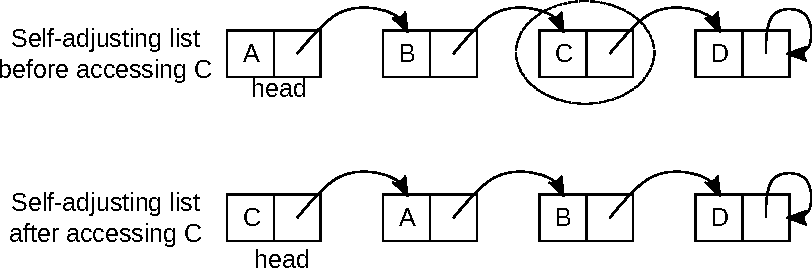
\includegraphics[width=.85\linewidth]{fig/mtf.pdf}
  \caption{A self-adjusting list containing nodes A,B,C and D serves the request to C and moves C to the front of the list to speed up future accesses to C.}
  \label{fig:mtf-example}
\end{figure}

Classic applications of MTF lists are information retrieval systems, compression~\cite{BentleySTW86}, etc. In general, any use case is a potential candidate application for MTF where the task is to match a request against a list of complex rules that do not lend themselves readily to be arranged into a fast lookup structure (e.g., a search tree), like inference in explainable rule-based AI and expert systems \cite{dovsilovic2018explainable}, rule matching in OpenFlow and P4 reference software switches \cite{openflow}, packet classification in networking (see later), etc.  We note that caching is a subset of list lookup, in that every algorithm for list reorganization gives rise to a different cache management algorithm \cite{SleatorT85}.  

\noindent%
\textbf{Search trees.} %
A search tree is an efficient tree data structure for locating specific keys from within an ordered set. A \emph{splay tree} is a self-adjusting version of a static search tree, in that it can dynamically reorganize itself by moving popular items closer to the root of tree and less frequently accessed elements to the bottom, while keeping the tree relatively well-balanced \cite{SleatorT85Splay, BoseDL08, Avin0020}. Since access time in a search tree is determined by the depth at which the requested item is to be found, splay trees can improve future access to the same or similar items when the input exhibits temporal or spatial locality (see Fig.~\ref{fig:bst_root_3}).  Note that a red-black tree, an AVL tree or any similar self-balancing tree is only partially ``self-adjusting'', in that it can rearrange only with respect to the items \emph{stored} in it but not with respect to the queries \emph{posed} to it.

\begin{figure}
 \centering
 \begin{tikzpicture}[level distance=30pt,
   level 1/.style={sibling distance=30pt},
   level 2/.style={sibling distance=30pt},
   level 3/.style={sibling distance=30pt}]
   % Left
   \node[circle,draw,minimum size=0.5cm,inner sep=1pt] (3a) {3}
   child {node[circle,draw,minimum size=0.5cm,inner sep=1pt] (2a) {2}}
   child {node[circle,draw,minimum size=0.5cm,inner sep=1pt] (5a) {5}
     child {node[circle,draw,minimum size=0.5cm,inner sep=1pt] (4a) {4}}
     child {node[circle,draw,minimum size=0.5cm,inner sep=1pt] (6a) {6}}
   };
   % Right
   \node[circle,draw, minimum size=0.5cm, inner sep=1pt] (4b) at (5.5,0) {4}
   child {node[circle,draw,minimum size=0.5cm,inner sep=1pt] (3b) {3}
     child {node[circle,draw,minimum size=0.5cm,inner sep=1pt] (2b) {2}}
     child[missing] {}
   }
   child {node[circle,draw,minimum size=0.5cm,inner sep=1pt] (5b) {5}
     child[missing] {}
     child {node[circle,draw,minimum size=0.5cm,inner sep=1pt] (6b) {6}}
   };
   % Arrow
   \node (draw=none) at (2.8,-1.5) [font=\large]{$\Rightarrow{Find(4)}\Rightarrow$};
 \end{tikzpicture}
 \caption{Splay-tree with elements 2, 3, 4, 5, 6. After accessing node 4 it is moved to the root that makes a subsequent lookup to it faster, while the tree is kept almost perfectly balanced.}
 \label{fig:bst_root_3}
\end{figure}

\begin{figure*}[t]
  % \begin{tabularx}{\textwidth}{D *{2}{s}}
  \begin{tabular}{m{.3\textwidth} m{.3\textwidth} m{.3\textwidth}}
  % \begin{tabular}{ccc}
    \hspace{28pt}\begin{tikzpicture} 
  \begin{axis}[%
    height=45pt,
    hide axis,
    xmin=10,
    xmax=50,
    ymin=0,
    ymax=0.4,
    legend style={
      draw=white!15!black,
      legend cell align=left,
      legend columns=2,
      font=\footnotesize}
    ]
    \addlegendimage{black,mark=*}
    \addlegendentry{Locality-boosting load balancer + Self-adjusting algorithm}
    \addlegendimage{black,mark=+}
    \addlegendentry{Locality-boosting load balancer + Static algorithm}
    \addlegendimage{black,mark=o}
    \addlegendentry{Roundrobin load balancer + Self-adjusting algorithm}
    \addlegendimage{black,mark=square}
    \addlegendentry{Roundrobin load balancer + Static algorithm}
  \end{axis}
\end{tikzpicture}

%%% Local Variables:
%%% mode: latex
%%% TeX-master: "../distributed_mrf"
%%% End:
\\
    \multirow{-6.4}{*}{\subcaptionbox{List lookup/uniform input\label{fig:multicore-list-uniform}}{\begin{small}
  \begin{tikzpicture}
    \begin{axis}[
      width=165pt,
      height=322pt,
      xlabel={number of CPU cores},
      x label style={at={(0.5,0.01)}},      
      ylabel={Speedup},
      y label style={at={(0.05,0.5)}},      
      xmin=1,
      xmax=48,
      xtick={1,12,24,36,48},
      ymin=0,
      ymax=3300,
      legend style = {
        anchor = north west,
        at = {(0.01, 1.01)},
        font=\tiny,
        % draw = none,
      },
      % scaled y ticks=false
      % no markers
      ]
      % use TeX as calculator:
      \addplot[black,mark=*] table[x=thread,y=speedup,] {fig/list/uniform-100k/multicore_mtf_modulo_uniform.txt};
      % \addlegendentry{Move-to-front/Local LB}
      \addplot[black,mark=+] table[x=thread,y=speedup,each nth point={3}] {fig/list/uniform-100k/multicore_linkedlist_modulo_uniform.txt};
      % \addlegendentry{Linked-list/Local LB}
      \addplot[black,mark=o] table[x=thread,y=speedup,each nth point={3}] {fig/list/uniform-100k/multicore_mtf_roundrobin_uniform.txt};
      % \addlegendentry{Move-to-front/Non-local LB}
      \addplot[black,mark=square] table[x=thread,y=speedup,each nth point={3}] {fig/list/uniform-100k/multicore_linkedlist_roundrobin_uniform.txt};
      % \addlegendentry{Linked-list/Non-local LB}
    \end{axis}
  \end{tikzpicture}
\end{small}

%%% Local Variables:
%%% mode: latex
%%% TeX-master: "../../../distributed_mrf"
%%% End:
}}%
    & \hspace{8pt}\subcaptionbox{List lookup/Zipf input\label{fig:multicore-list-zipf}}{\begin{small}
  \begin{tikzpicture}
    \begin{axis}[
      width=165pt,
      height=322pt,
      xlabel={number of CPU cores},
      x label style={at={(0.5,0.01)}},      
      ylabel={Speedup},
      y label style={at={(0.05,0.5)}},      
      xmin=1,
      xmax=48,
      xtick={1,12,24,36,48},
      ymin=0,
      ymax=3300,
      legend style = {
        anchor = north west,
        at = {(0.01, 1.01)},
        font=\tiny,
        % draw = none,
      },
      % scaled y ticks=false
      % no markers
      ]
      % use TeX as calculator:
      \addplot[black,mark=*] table[x=thread,y=speedup,] {fig/list/uniform-100k/multicore_mtf_modulo_uniform.txt};
      % \addlegendentry{Move-to-front/Local LB}
      \addplot[black,mark=+] table[x=thread,y=speedup,each nth point={3}] {fig/list/uniform-100k/multicore_linkedlist_modulo_uniform.txt};
      % \addlegendentry{Linked-list/Local LB}
      \addplot[black,mark=o] table[x=thread,y=speedup,each nth point={3}] {fig/list/uniform-100k/multicore_mtf_roundrobin_uniform.txt};
      % \addlegendentry{Move-to-front/Non-local LB}
      \addplot[black,mark=square] table[x=thread,y=speedup,each nth point={3}] {fig/list/uniform-100k/multicore_linkedlist_roundrobin_uniform.txt};
      % \addlegendentry{Linked-list/Non-local LB}
    \end{axis}
  \end{tikzpicture}
\end{small}

%%% Local Variables:
%%% mode: latex
%%% TeX-master: "../../../distributed_mrf"
%%% End:
}
    & \subcaptionbox{List lookup/uniform/single-core\label{fig:singlecore-list-uniform}}{\begin{small}
  \begin{tikzpicture}
    \begin{axis}[
      width=250pt,
      height=170pt,
      xlabel={\#thread},
      ylabel={Goodput [million req/sec]},
      xlabel near ticks,
      ylabel near ticks,
      xmin=1,
      xmax=26,
      ymin=0,
      % ymax=10,
      legend style = {
        anchor = north west,
        at = {(0.01, 1.01)},
        font=\scriptsize,
        % draw = none,
      },
      % no markers
      ]
      \addplot[black,mark=*] table[
      x=thread,
      y expr=\thisrowno{4}/1000000
      ]{fig/list/uniform-10/singlecore_mtf_modulo_uniform.txt};
      \addlegendentry{MTF w/ hash-based lb}
      \addplot[black,mark=+] table[
      x=thread,
      y expr=\thisrowno{4}/1000000
      ]{fig/list/uniform-10/singlecore_linkedlist_modulo_uniform.txt};
      \addlegendentry{Static list w/ hash-based lb}
      \addplot[black,mark=o] table[
      x=thread,
      y expr=\thisrowno{4}/1000000
      ]{fig/list/uniform-10/singlecore_mtf_roundrobin_uniform.txt};
      \addlegendentry{MTF w/ round robin lb}
      \addplot[black,mark=square] table[
      x=thread,
      y expr=\thisrowno{4}/1000000
      ]{fig/list/uniform-10/singlecore_linkedlist_roundrobin_uniform.txt};
      \addlegendentry{Static list w/ round robin lb}
    \end{axis}
  \end{tikzpicture}
\end{small}

%%% Local Variables:
%%% mode: latex
%%% TeX-master: "../../../hotnets22"
%%% End:
}
    \\
    & \hspace{8pt}\subcaptionbox{Cache lookup/uniform input\label{fig:multicore-cache-uniform}}{\pgfplotsset{
  RatePlot/.style = {
    tick pos = left,
    xtick align=outside,
    ytick align=outside,
    xlabel near ticks,
    ylabel near ticks,
    width=.4\textwidth,
    height=.3\textwidth,
    legend pos = north west,
    legend cell align=left,
    ylabel = {Throughput [Mpps]},
    xlabel = {number of CPU cores},
    xmin=1, xmax=32,
    ymin=0,
  },
  SpeedupPlot/.style = {
    RatePlot,
    ylabel={Speedup},
  },
  ClassBenchGroupPlot/.style = {
    group/group size = 1 by 2,
    group/horizontal sep = 0pt,
    group/vertical sep = 28pt,
  },
  ClassBenchRatePlot/.style = {
    RatePlot
  },
  ClassBenchSpeedupPlot/.style = {
    SpeedupPlot,
  }
}

%%% Local Variables:
%%% mode: latex
%%% TeX-master: "../distributed_mrf.tex"
%%% End:

%
\begin{small}
  % \tikzmath
  % {
  %   function est(\x)
  %   {
  %     if (\x < 10) then
  %     {
  %       return 0.1+0.9*(0.1*\x +(1-0.1*\x)*10)/\x;
  %     } else {
  %       return 0.1 + 0.9//\x;
  %     };
  %   };
  %   \a = est(4);
  %   \b = est(14);
  % }
  \begin{tikzpicture}
    \begin{axis}[
      width=165pt,
      height=120pt,
      xlabel={\#CPU cores},
      x label style={at={(0.5,0.04)}},
      ylabel={Speedup},
      % xlabel near ticks,
      % ylabel near ticks,
      y label style={at={(0.1,0.5)}},
      xmin=1,
      xmax=35,
      ymin=0,
      xtick={1,10,20, 30},
      % ymax=10,
      legend style = {
        anchor = north west,
        at = {(0.01, 1.01)},
        font=\scriptsize,
        % draw = none,
      },
      % no markers
      ]
      \addplot[SelfAdjustingSimMark,mark size=2pt] table[x=thread,y=speedup,each nth point={3}]{fig/cache/uniform-50k-2/mcore_cache_modulo_uniform.txt};
      % \addlegendentry{Local LB}
      \addplot[SelfAdjustingSimMark,mark=pentagon*,mark size=3pt,each nth point={3}] table[x=thread,y=speedup,each nth point={2}]{fig/cache/uniform-50k-2/mcore_cache_roundrobin_uniform.txt};
      % \addlegendentry{Non-local LB}
      % \addplot[domain=1:25,black,dashed]{x};
      % \addlegendentry{Linear scaling}
      % \addplot[domain=1:25,black,densely dotted]{1/(0.03+0.97/x)};
      % \addlegendentry{Amdahl's law}
      % \addplot[domain=0:25,black,densely dotted]{est(1.0)/est(x)};
      % \node at (100,100) {\a\b};
      % \addlegendentry{T}
      % \addplot[black,mark=o] table[x=thread,y=rate] {fig/cache/uniform-50k/multicore_cache_roundrobin_uniform.txt};
      % \addlegendentry{Round robin lb}
      % \addplot[black,mark=square] table[x=thread,y=rate] {fig/cache/uniform-50k/multicore_scache_roundrobin_uniform.txt};
      % \addlegendentry{staticcache / roundrobin}
    \end{axis}
  \end{tikzpicture}
\end{small}

%%% Local Variables:
%%% mode: latex
%%% TeX-master: "../../../distributed_mrf"
%%% End:
}
    & \subcaptionbox{Tree lookup/uniform input\label{fig:singlecore-tree-uniform}}{\pgfplotsset{
  RatePlot/.style = {
    tick pos = left,
    xtick align=outside,
    ytick align=outside,
    xlabel near ticks,
    ylabel near ticks,
    width=.4\textwidth,
    height=.3\textwidth,
    legend pos = north west,
    legend cell align=left,
    ylabel = {Throughput [Mpps]},
    xlabel = {number of CPU cores},
    xmin=1, xmax=32,
    ymin=0,
  },
  SpeedupPlot/.style = {
    RatePlot,
    ylabel={Speedup},
  },
  ClassBenchGroupPlot/.style = {
    group/group size = 1 by 2,
    group/horizontal sep = 0pt,
    group/vertical sep = 28pt,
  },
  ClassBenchRatePlot/.style = {
    RatePlot
  },
  ClassBenchSpeedupPlot/.style = {
    SpeedupPlot,
  }
}

%%% Local Variables:
%%% mode: latex
%%% TeX-master: "../distributed_mrf.tex"
%%% End:

%
\begin{small}
  \begin{tikzpicture}
    \begin{axis}[
      width=165pt,
      height=120pt,
      xlabel={\#CPU cores},
      x label style={at={(0.5,0.04)}},
      ylabel={Speedup},
      y label style={at={(0.1,0.5)}},
      xmin=1,
      xmax=36,
      xtick={1,10,20,30},
      ymin=0,
      % ymax=370,
      grid=major,
      tick pos = left,
      legend style = {
        anchor = north west,
        at = {(0.01, 1.01)},
        font=\scriptsize,
        % draw = none,
      },
      % scaled y ticks=false
      % no markers
      ]
      % use TeX as calculator:
      \addplot[SelfAdjustingSimMark,mark size=2pt] table[x=thread,y=speedup,each nth point={3}] {fig/tree/uniform-500/multicore_wsplay_modulo_uniform.txt};
      % \addlegendentry{Splay-tree/Local LB}
      \addplot[StaticSimMark,mark size=3pt] table[x=thread,y=speedup,each nth point={3}] {fig/tree/uniform-500/multicore_wbtree_modulo_uniform.txt};
      % \addlegendentry{B-tree/Local LB}
      \addplot[SelfAdjustingSimMark,mark=pentagon*,mark size=3pt] table[x=thread,y=speedup,each nth point={3}] {fig/tree/uniform-500/multicore_wsplay_roundrobin_uniform.txt};
      % \addlegendentry{Splay-tree/Non-local LB}
      \addplot[StaticSimMark,mark=square,mark size=3pt] table[x=thread,y=speedup,each nth point={3}] {fig/tree/uniform-500/multicore_wbtree_roundrobin_uniform.txt};
      % \addlegendentry{B-tree/Non-local LB}
    \end{axis}
  \end{tikzpicture}
\end{small}

%%% Local Variables:
%%% mode: latex
%%% TeX-master: "../../../distributed_mrf"
%%% End:
}
  % \end{tabularx}
  \end{tabular}
  \caption{Static vs. self-adjusting distributed systems scaling laws with round-robin and hash-based load balancing: (a) static vs. MTF list access speedup on uniform input ($m$=100k); (b) static vs. MTF list speedup on skewed input ($m$=100k, Zipf power law with $\alpha=1.01$), (c) static vs. MTF list access goodput with multiple threads running on a \emph{single core} for uniform input ($m$=10k); (d) cache access on uniform input ($m$=50k, $\delta=0.05$, $\rho=100k$ cycles); and (e) static balanced vs. splay tree speedup ($m=500$, $w=100k$ cycles).  Panels (a), (b), (d) and (e) show multicore speedup as the function of the number of CPU cores, each running a single worker, while (c) shows the single-core throughput (goodput) using an increasing number of lightweight parallel threads.}
  \label{fig:dist-self-adjusting-eval}
\end{figure*}

Splay trees are widely used to adaptively speed up associative memory and data compression algorithms \cite{jones1988application}, as well as a building block for more complex self-adjusting algorithms.

% Self-adjusting data structures are widely used in algorithms and computer systems, e.g., in computing point maxima and convex hulls~\cite{BentleyCL93}, organizing lists of identifiers in program compilation and interpretation~\cite{HesterH85}, detecting collisions in hash tables~\cite{HesterH85}, or compressing arbitrary input~\cite{BentleySTW86}. And indeed, every cache management scheme can be viewed as a self-adjusting data structure as well

\subsection{Superlinear scaling}
\label{sec:arch-scaling}

So how can locality-boosting load balancing and self-adjusting algorithms, when used together in a distributed system, produce superlinear scaling? Below we present an example, \emph{distributed self-adjusting list lookup}, along with a performance analysis as demonstration. Our architecture consists of a locality-boosting partitioning load-balancer (see Fig.~\ref{fig:locality-boosting-lb}) combined with a self-adjusting move-to-front list (see Fig.~\ref{fig:mtf-example}) implemented in the workers. The rationale for why this design achieves superlinear scaling is the following.

Suppose that there are $m$ items to be stored in the list and $k$ workers, each maintaining an independent index into the list. Suppose further that, at the input, requests can be received for any of the $m$ items. To make things more difficult we assume uniform request distribution on the system's input, which is, recall, the worst case for any self-adjusting algorithm by being totally \emph{unpredictable}. Thus, for a single worker move-to-front reordering has no useful effect and the worst case access time is $m$, identical to that of a static linked list.

Now suppose we move from 1 worker to $k$ parallel workers. This results that, within our architecture, the load balancer effectively partitions the uniformly distributed input on $m$ items into $k$ uniformly distributed input streams for only $\frac{m}{k}$ different items (see Fig.~\ref{fig:locality-boosting-lb}). This means that the workers' input features a much higher spatial locality than the system's input (which sports none).  Had we used a random or a round robin load balancer the workers would still see all the $m$ possible inputs, just with a sampled uniform distribution, and no locality. After a while, each MTF list in the workers will have its specific subset of $\frac{m}{k}$ items moved to the first $\frac{m}{k}$ positions (in an arbitrary order), reducing the worst-case lookup time from $m$ (1 worker) to $\frac{m}{k}$ ($k$ workers). This introduces $k\times$ speedup compared to the single-threaded case.

Then, superlinear speedup is merely a product of two simultaneous $k\times$ speedup factors: one $k\times$ speedup comes from the self-adjusting list getting progressively faster as we add new workers (recall the ``scaled size'' model from \S\ref{sec:backgound-dist-cache}), and another $k\times$ speedup because we extend the total compute capacity available to the system $k$ times. The effective speedup is then just the multiple of the two, yielding $k^2$ times speedup in total. Plugging into Amdahl's law we get the \emph{scaling law for distributed MTF lists} (see the scaling law in Fig.~\ref{fig:amdahl}):
\begin{equation}\label{eq:mtf-perf}
  S_l(k) = \frac{T_l(1)}{T_l(k)} = \frac1{s + \frac{1-s}{k^2}} \enspace .
\end{equation}

% We used this scaling law as the graphical illustration for superlinear scaling in Fig.~\ref{fig:amdahl}. 
For small values of $k$ we obtain $O(k^2)$ scaling, despite that uniform request distribution is the worst case for self-adjustments. This hints at a great future potential for networking workloads that typically exhibit highly skewed request distributions~\cite{832484}.

\subsection{Evaluation}
\label{sec:sims}

Fig.~\ref{fig:dist-self-adjusting-eval} presents the results from a comprehensive simulation study we conducted to understand distributed self-adjusting systems performance over a broad selection of load balancing policies, self-adjusting algorithms, and input distributions. The simulator was coded in roughly 1,000 lines of Go and uses lightweight threads (goroutines) managed by the Go runtime to run a given number of workers in parallel. We used a simple home-grown implementation for static and MTF lists and standard Go modules for LRU caches \cite{golang-lru}, static balanced trees \cite{golang-btree} and splay trees \cite{golang-splay}. In order to make tree lookup CPU bounded we used an ``expensive'' order underneath the tree, where every comparison operation costs a configurable $w$ number of extra cycles. The simulator creates the specified combination of a load balancer, $k$ worker threads running the selected lookup algorithm, and a random input sequence with a given request distribution, and then performs a configurable number of lookup operations and measures the total execution time with nanosecond precision. To obtain a full picture, the total execution time includes the transient time needed to warm up the self-adjusting algorithms running in the threads. For the specification of the evaluation platform, refer to \S\ref{sec:sa-nf-tables-eval}.

Our observations are as follows. First, it is immediate that \emph{the right combination of a locality boosting load balancer and a self-adjusting algorithm robustly delivers superlinear speedup}, irrespectively of the problem domain or the input distribution. Even for a worst-case uniform request distribution, we obtain $3,300\times$ speedup(!) for list access on 48 CPU cores, almost $70\times$ of ``ideal'' linear speedup, $200\times$ speedup on LRU caches and $65\times$ speedup on tree search with 36 CPU cores. Usually the superlinear growth is so dominant that we can hardly put the Amdahl's scaling on the same diagram.  Second, \emph{only the combination of locality-boosting load balancing and self-adjusting algorithms produces superlinear speedup}, all other combinations (i.e., round robin with any algorithm or static algorithm with any load balancer) fall back to Amdahl's scaling.  Third, \emph{self-adjustment clearly has its overhead}. This can be observed in Fig.~\ref{fig:singlecore-list-uniform}, which, instead of the relative speedup shows the absolute throughput. Here, the single-threaded self-adjusting version is clearly slower than the static version (a trait we identified in essentially all cases with uniform input). Fourth, \emph{the overhead of self-adjustment becomes irrelevant for more than one CPU core, or with skewed request distributions}. For instance on a Zipf input distribution (Fig.~\ref{fig:multicore-list-zipf}) even the single-threaded self-adjusting version is already $2$--$2.5\times$ faster in an absolute term irrespectively of the load balancer (not shown in the figure). However, \emph{only} combining with a locality-boosting load balancer it produces superlinear speedup.

And finally a rather surprising finding. In Fig.~\ref{fig:singlecore-list-uniform} we show an evaluation that was executed with an increasing number of parallel threads manually constrained to run with at most 110\% CPU utilization using \texttt{cpulimit}. This effectively simulates a single core worth of total CPU shared by \emph{all} the parallel workers, with a little surplus for the load balancer. The results indicate that the distributed self-adjusting system (but \emph{only} this combination!) delivers linear speedup with adding new threads. With uniformly distributed requests, we achieve $25\times$ speedup by spawning 25 parallel goroutines, each sharing a single CPU core.  And this is despite that the overhead of request generation, goroutine scheduling, and memory management all count towards the total system load and take away precious CPU time from the useful workload.

But how can parallelization benefit performance when we do not even add more CPU power to the system? Recall, in the multicore case superlinear speedup emerges thanks to the superposition of two independent $k\times$ speedup trends, one delivered by the self-adjusting workers and another added by us throwing $k\times$ more CPU power to the system. When the total available CPU is limited only first $k\times$ speedup factor is in effect, resulting in the observed linear scaling trend.

% glitches are cpu architecture specific

% LET's SKIP THIS: highly speculative!!!!!!!!!!!1
%
% \subsection{Revised Amdah's law}
% \label{sec:sims}

% An interpretation of superlinear scaling: if we introduce the notion of the ``virtual job size''. Implicit in Amdahl's law \eqref{eq:amdahl} is that the job size remains the same independently of $k$. Parallel self-adjustments, however, may actually \emph{decrease} the amount of work each worker has to perform per each request. Let $b(k)$ denote the ``virtual job size'' perceived by each worker when the number of  workers is $k$. We observe that in parallel self-adjusting systems $b(k)$ is decreasing in $k$; e.g., for MTF we have $b(k) = \frac1{k}$.

% \begin{equation}\label{eq:revised-amdahl}
% S(k) = \frac{T(1)}{T(k)} = \frac{1}{s + \frac{1-s}{k^{\alpha}}} \enspace .
% \end{equation}

% Amdah's law for $\alpha=1$, distributed MTF scaling for $\alpha=1$, superlinear scaling with $\alpha>1$

%%% Local Variables:
%%% mode: latex
%%% TeX-master: "distributed_mrf"
%%% End:



\section{Case-study }\label{sec:case-study}

Next, we present a case study for systematically applying the distributed self-adjusting systems architecture to a common networking problem: software packet classification \cite{gupta2001algorithms}. The goal is to demonstrate the general engineering methodology by assembling \emph{existing} techniques into a distributed self-adjusting scheme and understand when, and to what extent, superlinear scaling emerges. We consider it a success if we find at least one synthetic and one realistic workload that produces positive result (as we will see, we find way more). It is a stated \emph{nongoal} to conceive novel algorithms and present new capabilities, let alone to present the fastest ever software packet classifier implementation. % (that award undeniably goes to DPDK \texttt{rte\_acl} \cite{rte-acl})
Still, our multicore self-adjusting firewall will prove several times faster than the default Linux kernel implementation on a wide range of workloads.

Recall, to achieve superlinear scaling we have to combine a locality-boosting load balancer with a self-adjusting algorithm. There is a broad range of potential use cases that come with an adequate self-adjusting algorithm \cite{SleatorT85Splay, BentleyCL93, HesterH85, HesterH85, BentleySTW86, Avin0020, ParkM12}. Eventually, we stayed with packet classification for the following reasons.  First, packet classifiers possess an intrinsic linear lookup structure, where the filter rules defined by the administrator are matched in the order of priority for each packet. This makes packet classification an appealing candidate for applying the move-to-front heuristics (but see ramifications related to handling rule-dependencies below). Second, the default Linux firewall implementation, \nftables, performs a linear sweep of a static rule list ordered priority-wise for each packet. This will buy us the non-self-adjusting baseline for free. Third, there is an infamously difficult theoretical problem underlying packet classification \cite{10.1145/2619239.2626294,10.1006/jagm.1996.0063, PacutVAPRS2022, 10.1145/2619239.2626294, 10.1145/1851182.1851208, 10.1145/863955.863980, gupta2001algorithms, 10.1145/3359989.3365431}. Achieving superlinear speedup on such a hard problem poses a great challenge. Fourth, the Linux kernel network stack offers several flexible software and hardware based load balancers for dispatching packets to multiple parallel classifier instances running on different CPU cores \cite{rss-linux}. These readily support for 5-tuple hashing along with many other policies for obtaining a hash on the packet header fields, and we can easily reuse these to implement the locality boosting load balancer component. And fifth, there is a recently published geneal self-adjusting algorithm that lends itself to be implemented in \nftables for experimentally checking superlinear scaling right on the Linux kernel firewall \cite{10228937}.

\subsection{The Linux packet classier}
\label{sec:sa-pack-class}

Network firewalls, in general, are a means to control incoming and outgoing network traffic based on user-defined packet classifier rules. This is useful to improve security, control access, filter and protect against ongoing attacks, and log\slash monitor network activity. The Linux kernel contains several packet classifier implementations, the newest of which is \texttt{nftables}.

The main concept of a packet classifier is a \emph{rule}, which specify a pair of a filtering criteria and the corresponding actions. The filter is essentially a user-defined regular expression on specific fields of the packet header or metadata, and the action decides what to do for packets that match the filter (accept, drop, log, etc.). Chains are sequences of related rules, which must be matched in the order of priority (see Fig.~\ref{fig:class-dep}). When a packet enters a chain, it is compared against the rules in that chain. If there is a match, the corresponding is executed and the lookup is over. Otherwise, the next rule is matched priority-wise, and the linear search goes on until the first match is found.  The \nftables kernel engine adds a simple virtual machine that defines a DSL to inspect network packets and make decisions, which contains some optimization allowing multiple comparisons to be replaced with a single operation. This makes the \nftables packet classifier agnostic to the specifics of particular network protocols, in contrast to, e.g., \texttt{iptables}, which contains an embedded fixed protocol parser.

\begin{table}[t]
  \centering
  \begin{small}
    \renewcommand{\tabcolsep}{2pt}
    \begin{tabular}{r|l|l|r|r|l}
      \textbf{Prio} & \textbf{Proto} & \textbf{Src IP} & \textbf{Dst IP} & \textbf{Dst Port} & \textbf{Action}\\
      \hline
      1 & UDP & 192.168.178.33 & 23.0.0.45 & 53 & ACCEPT\\
      2 & TCP & 10.10.10.0/24 & 23.0.0.45 & 443 & DROP\\
      3 & TCP & 10.10.10.10/32 & 23.0.0.45 & ANY & ACCEPT\\
      4 & UDP & 192.168.178.0/24 & 23.0.0.45 & 53 & DROP\\
      5 & IP & 192.168.0.0/16 & 23.0.0.0/8 &  & ACCEPT\\
    \end{tabular}
  \end{small}%
  \caption{Sample firewall rule set}
  \label{fig:class-sample}
\end{table}

\subsection{Self-adjusting packet classification}
\label{sec:sa-sa-pack-class}

\begin{figure}[t]
  \centering
  \begin{small}
    \begin{tikzpicture}[->,>=stealth,node distance=2.5cm, auto, every node/.style={circle,draw,minimum size=0.5cm,inner sep=2pt}]
      % Branch 1
      \node[circle,draw] (5) {5};
      \node[circle,draw,right of=5] (4) {4};
      \node[circle,draw,right of=4] (1) {1};
      
      % Branch 2
      \node[circle,draw,below of=5,yshift = 1.5cm] (3) {3};
      \node[circle,draw,right of=3] (2) {2};
      
      % Edges
      \draw (5) -- (4);
      \draw (4) -- (1);
      \draw (3) -- (2);
    \end{tikzpicture}
  \end{small}
  \caption{Dependency graph}%
  \label{fig:class-dep}
\end{figure}

\begin{algorithm}
  \caption{Move Recursively Forward (MRF)}
  \label{alg:alg}
  \begin{small}
    \begin{algorithmic}[1]
      \Procedure{MRF}{$y$}
      \If{$y$ has no dependencies}
      \State Move $y$ to the front of the list
      \Else
      \State Let $z$ be the direct dependency of $y$
      \State Move node $y$ to position$(z) + 1$
      \State \Call{MRF}{$z$}
      \EndIf
      \EndProcedure
    \end{algorithmic}
  \end{small}
\end{algorithm}

\subsection{Locality boosting with RSS}
\label{sec:sa-rss}




\subsection{Implementation}
\label{sec:sa-nf-tables-impl}
In our case study, we focus on the \textit{nf\_tables} firewall within the Linux Kernel. First, we replace the static list used to store the rules with the self-adjusting RMF list. 
In order to achieve optimal scaling properties and avoid any lock contention, the ruleset is replicated for all CPUs. To distribute the network traffic across all cores, we use RSS hash filter options (\textit{rx-flow-hash}).
This generates a hash using the header fields within the network packet, which then dictates to which receive queue the packet is delivered.
We use Classbench \cite{4237157} to generate the rulesets and traffic traces with which we test our implementation using real-world resembling scenarios. 


\subsection{Evaluation}
\label{sec:sa-nf-tables-eval}

- synthetic microbenchmarks and realistic macrobenchmark: rulesets and traffic

% when superlinear scaling appears
\noindent%
\textbf{Superlinear scaling.} %  (3 figs + 1 with Jonas's stats?)
\begin{itemize}
\item no dependency rule-set and uniform traffic
\item rule-template: 1.2.3.4+udp-dst:i[1,n], where n is a parameter: 997, 4999, 10007 (primes)
\item flows: uniform + zipf: 20000 * packets=pcap
\item RSS: 5-tuple hash
\item one fig per rule size (packet rate): 4 plots: SA+uniform, SA+zipf, baseline+uniform,baseline+zipf
\item takeaway: rule size + traffic-locality do not matter (3 figs + 1 with Jonas's stats?)
\end{itemize}

% when superlinear scaling deteriorates into linear because SA does not work
\noindent%
\textbf{Active flow size.} %  (1 fig)
\begin{itemize}
\item same no-dep rule-set (udp-dst) + 5, 50, 500 flows per rule
\item RSS: 5-tuple hash
\item fig: 3 scaling laws, one for each active-flow-size: speedup (speedup: normalized for the single-core rate)
\item takeaway: the more the flow count the more rules are replicated across cores and the larger the working set size and superlinearity vanishes
\end{itemize}

\noindent%
\textbf{Rule dependencies.} % (1 fig)
\begin{itemize}
\item rule template: 1.2.3.4/{32,28,24,20,16,12,8,4,0}+udp-dst:i[1,500]
\item   traffic template: uniform: 1.2.3.4:i (500 flows) 
\item   3 rules-sets: small-dep (/0 and /32 for each chain), medium-dep (/{32,24,16,8,0}  for each chain), high-dep (/{32,28,24,20,16,12,8,4,0}  for each chain)
\item   RSS: 5-tuple hash
\item: fig: 3 scaling laws: speedup (normalized for the single-core rate)
\item takewaway: the more dependencies, the less superlinearity (dependencies must be in the working set at each thread)
\end{itemize}

\noindent%
\textbf{Locality boosting.} % (1 fig)
\begin{itemize}
\item benchmark the high-dep rule-set with different RSS hashes: bad hash: IP-dst(everything goes to 1 cpu, no scaling), 5-tuple hash (same as in the previous case), good hash: udp-dst hash (dep chains are partitioned across cpus: only a few chains per each CPU) 
\item  takeaway: load-balancing policy matters, the less locality-boosting, the less superlinearity
\end{itemize}

% realistic macrobenchmark
\noindent%
\textbf{Real workload.} % (3 figs)
classbench: the good news (3 figs with 3 different seeds + 5000 rules) + throughput and latency diagrams

%%% Local Variables:
%%% mode: latex
%%% TeX-master: "distributed_mrf"
%%% End:



\section{Related work}
\label{sec:related-work}

\noindent%
\textbf{Locality boosting load balancing.} %
\begin{itemize}
\item NICs increasingly used to intelligently move data between the network, CPU, GPU and accelerators \cite{sherry-ccr23}
\item Linux contains a comprehensive toolset to tune the way packets are dispatched to CPUs \cite{rss-linux}
\item plain RSS is static, RSS++ is a load and state-aware receive side scaling mechanism aiming to keep CPU load constant \cite{10.1145/3359989.3365412}
\item Reframer can be used to reorder packets for improving temporal locality \cite{276946,246322}
\item rule partitioning: Hicuts \cite{820051}, Hypercuts \cite{10.1145/863955.863980}, Efficuts \cite{10.1145/1851182.1851208}, CutSplit \cite{8485947} build a decision tree, with each node representing a ``cut'' of the rule-space, whose leaf nodes store only a small number of rules. A linear search among these rules yields the desired matching. The cuts are designed so that the rule lists in the leaves are as small as possible, with the least possible rules replicated in multiple lists. We argue that these cuts could be reused in our multicore classifier to partition the rule set, and represented in the NIC as Receive Flow Steering (RFS) filters
\item In fact, our classifier can be viewed as a parallel extension to these schemes, just with ``dumb'' hash-based cuts for traversing the decision tree in one step and maintaining the rule lists in the leaves in a self-adjusting list. It is a surprising finding that such a simple extension of Hicuts \cite{820051}, Hypercuts \cite{10.1145/863955.863980}, Efficuts \cite{10.1145/1851182.1851208}, CutSplit \cite{8485947} can yield superlinear scaling
\end{itemize}

\noindent%
\textbf{Self-adjusting data structures.} %
\begin{itemize}
\item Self-adjusting data structures are widely used in algorithms and computer systems
\item simplest SA algorithms are caches; often used in distributed computing: predictive state caching in NFs \cite{295537}, SQL caches: redis, memcached \cite{10.5555/1012889.1012894, 180324}, distributed web caching and CDNs \cite{295603}, dataplane kv store caching \cite{ghigoff2021bmc}, query result caching in microservices \cite{295493}
\item to what extent these achieve superlinear scaling is an open question
\item MTF: building block of a self-adjusting algorithm for computing point maxima and convex hulls \cite{BentleyCL93}, program compilation and interpretation \cite{HesterH85}, detecting collisions in hash tables~\cite{HesterH85}, and data compression \cite{BentleySTW86}
\item the problem of cache management can be viewed as a self-adjusting list rearrangement problem \cite{SleatorT85}
\item further self-adjusting data structures include splay trees \cite{SleatorT85Splay}, self-adjusting skip lists \cite{BoseDL08}, push-down trees \cite{Avin0020}, or self-adjusting trees for storing geometric data \cite{ParkM12}
\item these are all candidates to be used, along with a proper locality boosting load balancer, to reach superlinear scaling in distributed applications
\end{itemize}

\noindent%
\textbf{Superlinear scaling.} %
\begin{itemize}
\item applications: database systems \cite{scalability-analyzed, 10.5555/1012889.1012894}, SDN analytics \cite{sdn-analytitcs}, high-performance computing \cite{556383, 7733347, 6483679}, multi-robot systems \cite{10.1007/978-3-319-77610-1}, and parallel search in information retrieval systems \cite{dobb-1, dobb-2}
\item full taxonomies in \cite{7733347, 80148}
\item two ways to achieve such superlinear speedup \cite{7733347, 80148}: do disproportionately less work in each worker as we scale the system \cite{7733347}, or add more resources per thread \cite{80148}
\item distributed caching \cite{271208, dobb-2} is a variant of the second: the more parallel workers the more cache space available, which tends to make memory-bound\slash cache-bound code disproportionately faster \cite{80148}
\item non-persistent algorithms, which finish when one of the workers finds the solution, often cause a ``spurious superlinear'': our SA scheme does not belong to this category, since a single packet is always fully matched at a single worker \cite{7733347}
\item counter arguments: impossible \cite{10.1016/0167-8191(86)90024-4}, complete dismissal by the father of the ``Universal Scalaility Law'' \cite{gunther-hotsos, 10.1145/2773212.2789974}
\item never reported in networked application as far as we are aware of + ours is the first general design methodology to achieve it
\item superlinear growth is often found in nature, e.g., describing the scaling of human communities to large cities \cite{PhysRevE.79.016115}
\end{itemize}

%   Models of self-adjusting data structures are based on the cost of access and rearrangement. For example:

%   \begin{enumerate}
%   \item \textbf{Self-adjusting lists}~\cite{SleatorT85}. We are given a set of items, arranged in a linear list, and a sequence of access requests $\sigma$ to the nodes of the list.
%     Upon receiving an access request to a node in
%     the list, an algorithm searches linearly through the list, starting
%     from the head of the list, traversing nodes until encountering the
%     accessed node. Accessing the node at position i in the list costs i
%     (the first node is at position 1).
%     After serving a request, an algorithm may
%     choose to rearrange the nodes of the list, paying the cost 1 per each transposition of neighboring items. 


%   \item \textbf{Binary search trees}~\cite{SleatorT85Splay}.
%     When the universe of items is ordered, we may store them in a binary search tree.
%     A classic binary search tree is a \emph{splay tree}~\cite{SleatorT85Splay}.
%     Another important search tree is $O(\log \log n)$-competitive \emph{tango tree}~\cite{demaine2007dyynamic}.
%     The dynamic optimality conjecture~\cite{SleatorT85Splay} (does an $O(1)$-competitive algorithm exist?) is a major unresolved question, in contrast to the simpler self-adjusting lists setting.
%     Splay trees have other properties, e.g. working set bounds, static optimality~\cite{SleatorT85Splay} and other.



%   \item \textbf{Other self-adjusting data structures}. 
%     Self-adjusting skip lists~\cite{BoseDL08} have an equivalent of the working set bound of splay trees.
%     Push-down trees~\cite{Avin0020} are dynamically optimal and have the working set bound.
%     Adaptive geometric space partitioning data structures exist, e.g. self-adjusting trees for storing geometric data~\cite{ParkM12}.
%     The online metrical task system model~\cite{Borodin1992} underpins all these models, and captures generalizations such as caching, which has self-adjusting algorithms such as LRU~\cite{SleatorT85}.
%   \end{enumerate}


% %   Other examples: intrusion detection as mtflist, flow table lookup as splay tree, etc.
% %   Each have their own challenges, and our model is just an example.

%   \paragraph*{Locality.}
%   Common inputs have high locality, i.e. the same items are accessed repeatedly.
%   The locality parameter of input is often the determining factor for the performance of self-adjusting data structures (e.g. there exist arguments of locality for self-adjusting lists~\cite{AlbersL16}, working set bounds for splay trees~\cite{SleatorT85Splay} and paging~\cite{AlbersFG05}).


%   \subsection{Load Balancing and Scaling}

%   \paragraph*{Load balancing with random hash functions.}
%   A random load balancing assignment function is sufficient to load-balance correctly.
%   Gonnet~\cite{Gonnet81} proved that when throwing $n$ balls uniformly and independently at random into $n$ bins, the fullest bin has
%   load $(1 + o(1)) \log n/ \log \log n$ in expectation.
%   The maximum bin load with this approach is $O(\log n/ \log \log n)$ with high probability~\cite{DubhashiR98}.

%   \paragraph*{Practical load balancing.}
%   RSS+ paper~\cite{10.1145/3359989.3365412}.

%   \subsection{Packet classification}

%   Various data structures for packet classification were proposed in the literature: lists, tries, hash tables, bit vectors, or decision trees~\cite{gupta2001algorithms,Srinivasan1999,Eppstein2001}, as well as hardware solutions (TCAM).
%   Packet classifiers are often accompanied by caching systems that provide some adjustability to traffic.
%   Due to its simplicity, a~linear lookup structure is commonly applied in practice, e.g., in the default firewall suite of the Linux operating system kernel called \texttt{iptables}~\cite{MianoBRBLP19}, the OpenFlow reference switch~\cite{openflow}, and in many QoS classifiers.


%%% Local Variables:
%%% mode: latex
%%% TeX-master: "distributed_mrf"
%%% End:



% !TEX ROOT = ./distributed_mrf.tex
\section{Conclusions}\label{sec:conclusions}

In this paper, we present theoretical and empirical proof that locality-boosting load balancing combined with parallel self-adjusting algorithms together yield faster-than-linear speedup in many applications on a wide range of workloads. Our main contribution not necessarily stands in that we show that superlinear speedup \emph{exists} (this has been known for quite some time), but rather that we identify the main architectural patterns commonly appearing in the use cases where it was genuinely observed and synthesize these into a comprehensive and universal design methodology to \emph{reproduce} it. This methodology is then used in extensive simulations, producing an order of magnitude faster scaling than previously observed. We extend the default \nftables Linux subsystem into a true self-adjusting packet classifier, which we use to identify the main workload characteristics (rule-dependency, flow diversity) that affect superlinear growth trends.  Future research will be needed to apply our methodology in a broader range of use cases: for instance, rule-based network intrusion detection systems like Snort or Suricata \cite{10.5555/2537857.2537883} or explainable AI inferencing seem like appealing application candidates.

%%% Local Variables:
%%% mode: latex
%%% TeX-master: "distributed_mrf"
%%% End:



%%%%%%%%%%%%%%%%%%%%%%%%%%%
% \section{Acknowledgments}
\label{sec:ack}

thank E/// for the lab!

%%% Local Variables:
%%% mode: latex
%%% TeX-master: "distributed_mrf.nsdi"
%%% End:



\bibliographystyle{abbrv} 
\begin{small}
\bibliography{mrf}
\end{small}

\end{document}

  
